Many beyond-SM scenarios involve an extended Higgs sector. For example, in Two-Higgs-Doublet-Models (2HDMs) one additional Higgs doublet is  introduced,
resulting in a total of five physical states: two CP-even scalars ($h$ and $H$, corresponding to the light and heavy states, respectively),
a CP-odd scalar (i.e. pseudo-scalar) ($A$), and two charged scalars ($H^{\pm}$). The light CP-even scalar ($h$) is taken to be the SM Higgs boson. A generic CP-conserving 2HDM with natural flavour conservation, and a lighter CP-even Higgs boson playing the role of the SM Higgs boson, has five free parameters: three Higgs boson masses ($m_H$ , $m_A$, $m_{H^{\pm}}$), the mixing angle of the two CP-even Higgs fields ($\alpha$), and the ratio of the vacuum expectation values of the two Higgs doublets ($\tan{\beta}$). Existing constraints from direct searches for heavy neutral bosons by the ATLAS and CMS Collaborations, as well as precision measurements of the production cross-sections and decay rate of the SM Higgs boson, restrict the available parameter-space to the so-called ‘alignment limit’, $\sin{\beta-\alpha}\rightarrow 1$. In this limit the $h$ couplings are the same as for the SM Higgs boson.

This search is focused on the production of heavy neutral bosons in association with two top quarks,
and with subsequent decay into two top quarks: \ttHA. An example of Feynman diagram is shown in Fig.~\ref{fig:dia}. 
From generator level studies\footnote{See: https://its.cern.ch/jira/browse/ATLMCPROD-2848 \\ https://its.cern.ch/jira/browse/ATLMCPROD-2419 , https://its.cern.ch/jira/browse/ATLMCPROD-2422.} is known that the kinematic of the processes involving the production of a CP-even or a CP-odd Higgs boson with same mass are very similar (see Appendix~\ref{app:t_channel}); only the cross sections change. 
Therefore processes involving a scalar heavy Higgs boson are also used to model processes involving the production of a pseudo-scalar.

\begin{figure}[tbp]
  \begin{center} \setlength{\tabcolsep}{2.5pt}\footnotesize
    \begin{tabular}{c}
	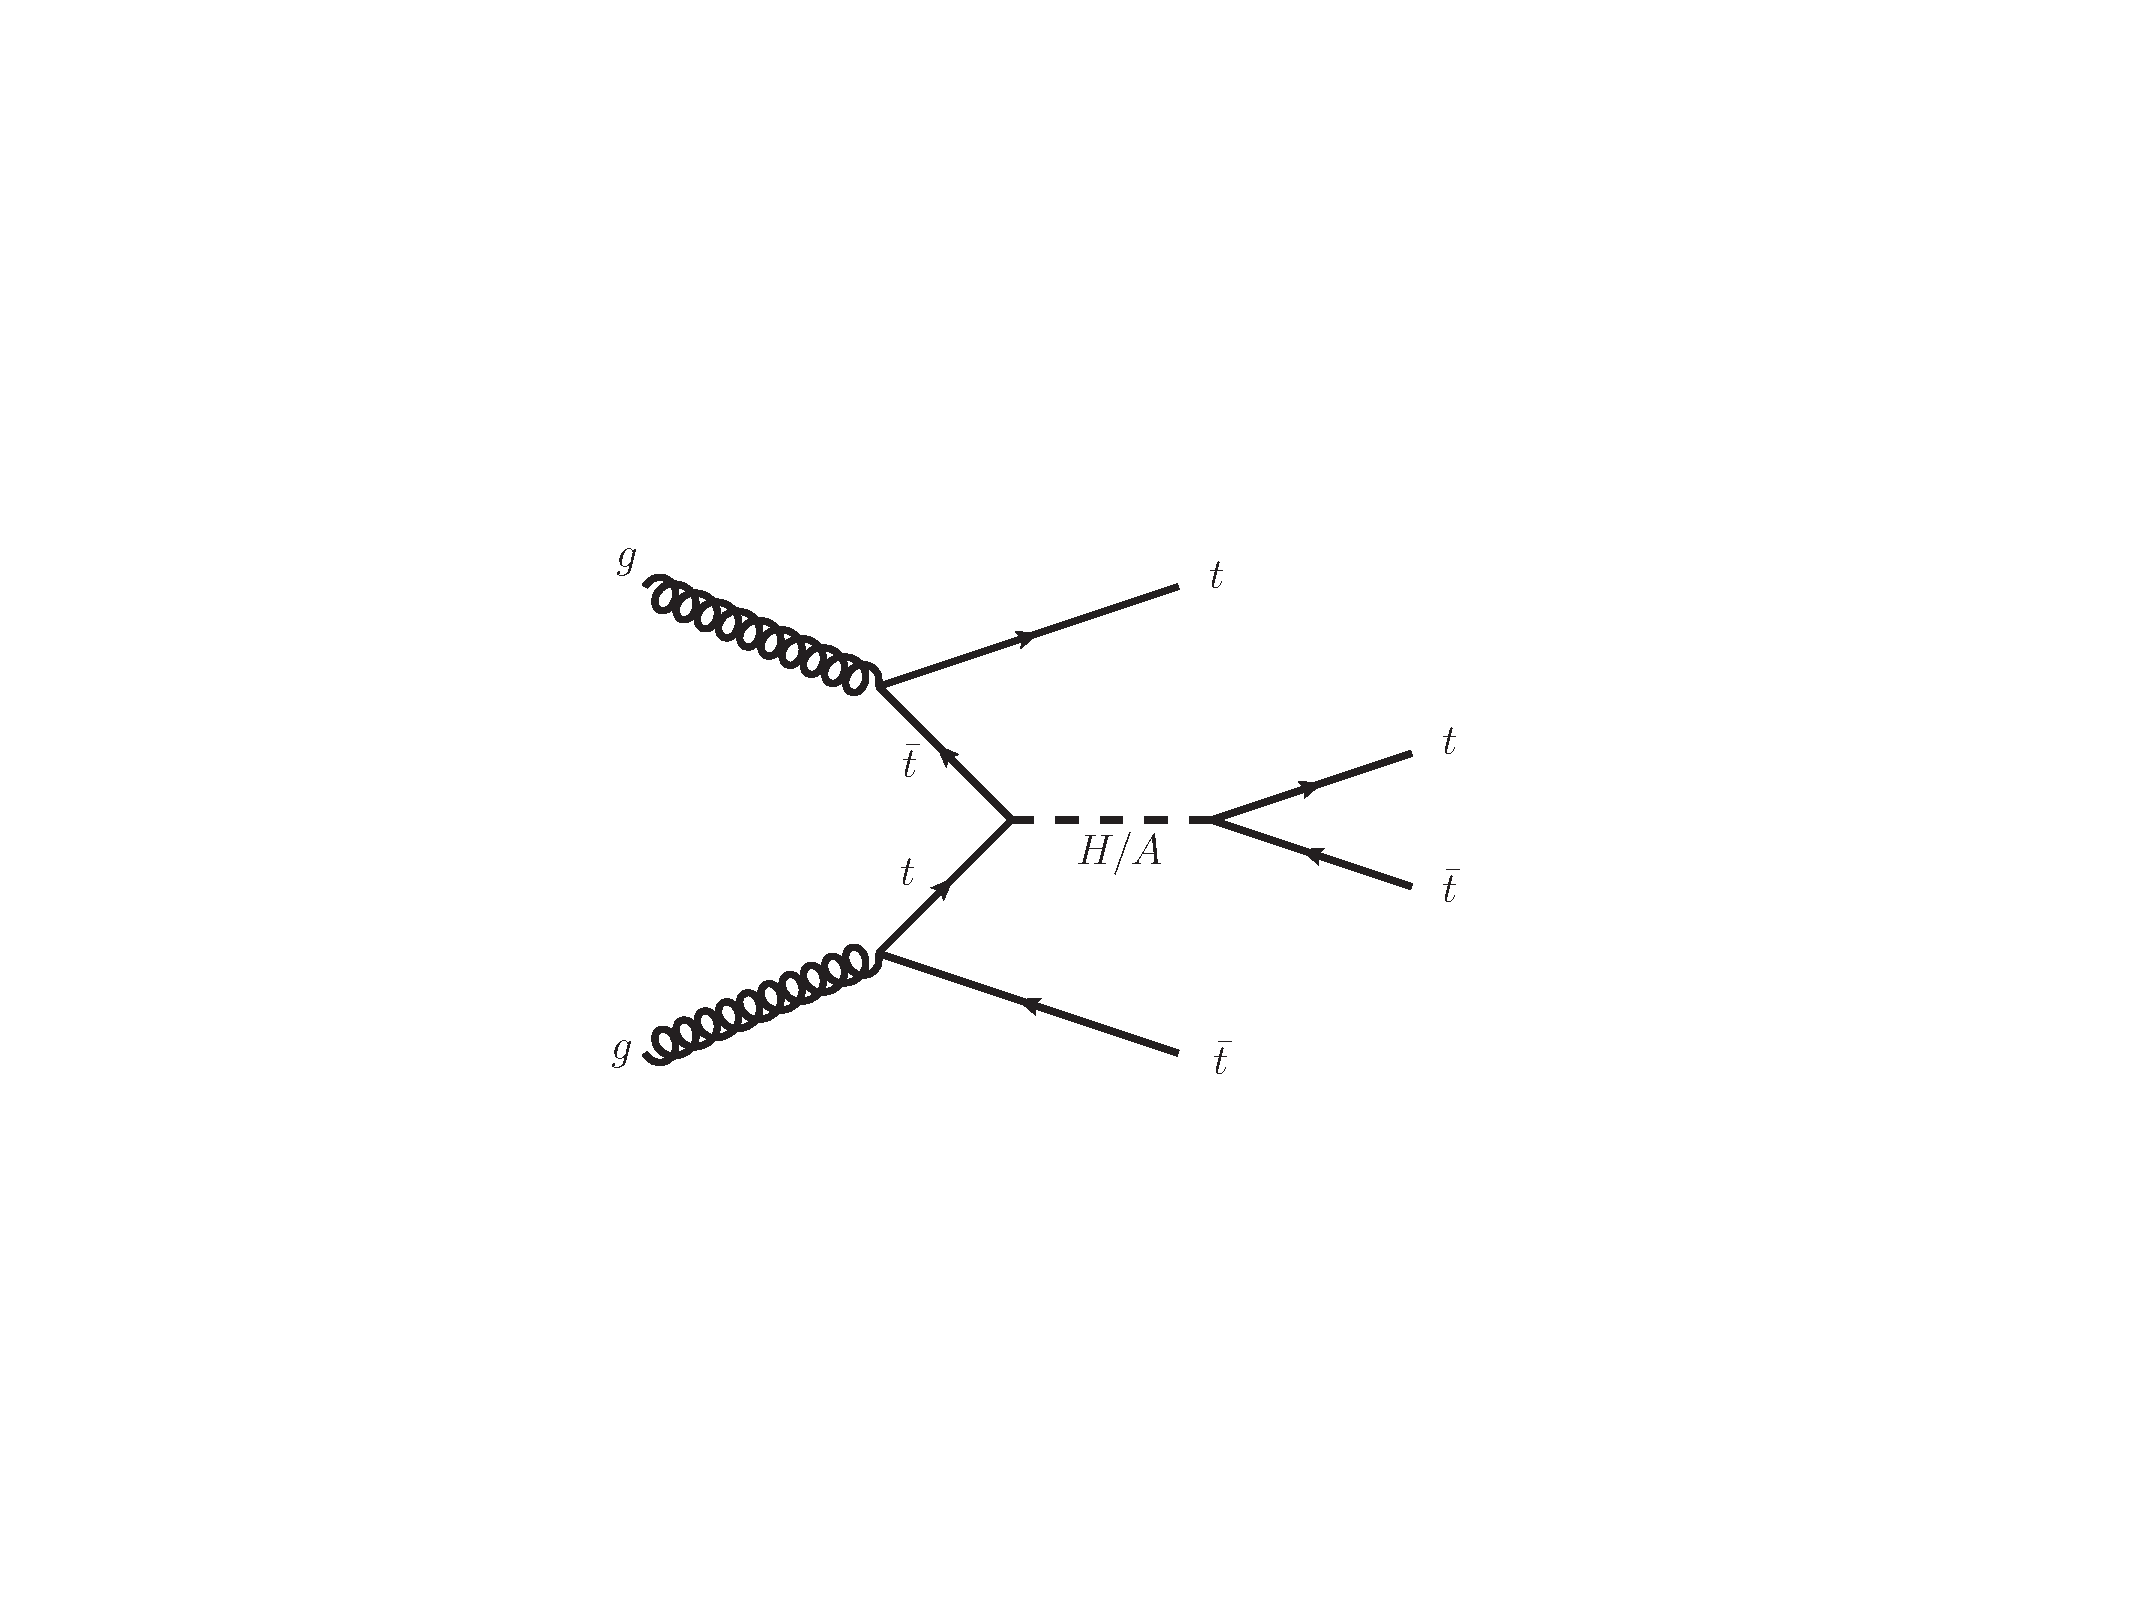
\includegraphics[width=0.43\textwidth]{figures/signal_modeling/hbsm_dia_tth.pdf} \\
    \end{tabular}
     \caption{Example of Feynman diagram for \ttH\ production; the diagrams involving the production of a CP-odd Higgs boson are equivalent.}
   \label{fig:dia}
  \end{center}
\end{figure}

The \ttH\ signal is generated in Type-II 2HDM.  

The signal MC samples are used to describe the kinematics of the signal processes of interest, and they are 
normalised according to the benchmark cross sections described in Sect.~\ref{sec:signal_cross_sections}.

\subsection{Signal generation details}

The signal generation is performed at leading order with \MadG\ from the AtlasProduction release 19.2.5.38.\footnote{https://twiki.cern.ch/twiki/bin/viewauth/AtlasProtected/MadGraph5aMCatNLOForAtlas\#Release\_history}. Only the production via the $s$-channel is considered. The impact of the $t$-channel has been documented in  Appendix~\ref{app:t_channel}. Although the impact on the final results was not investigated, the impact on kinematic distributions was found to be around 10\%, and the $t$-channel has been neglected in this search. All the signal samples are normalised to a cross section of 12 fb. This is the excess between the ATLAS measurement of the cross section of the SM four-top-quark production (24 fb) \cite{Aad:2020klt} and the SM prediction of four-top-quark production (12 fb). This signal normalization is used in the blinding strategy in which we blind all bins with $S/B>5\%$.

The samples are generated in 2HDM-typeII as implemented in the \MadG\ generator\footnote{http://atlas.web.cern.ch/Atlas/GROUPS/COMPUTING/links/releaseDirectory/19.2.5/madgraph/MG5\_aMC\_v2\_3\_3/models/2HDMtypeII/}.
The generated Monte Carlo samples use $\beta=10$ [rad.] and no mixing between the H/A-bosons, therefore the H/A bosons are simultaneously mass and CP eigenstates.
At leading order the kinematics of the investigated BSM processes doesn't depend on the value of $\beta$ coupling, this was confirmed by truth level 
studies~(see Appendix~\ref{app:tan_beta_dep}).
%~\footnote{This was documented on slide 14\\ https://indico.cern.ch/event/479524/contributions/1999037/attachments/1217207/1777909/h\_to\_fermions\_meeting\_2.pdf.}.

The matrix-element calculation is performed at leading order in four-flavour-number scheme and takes into account the spin correlation of all decay products of the W-bosons and top-quarks. The four-flavour parton distribution function set NNPDF31$\_$lo$\_$as$\_$0118 PDFs. is used. \MadG\ is interfaced to \pythiaeight\ for the parton-shower, hadronisation and underlying event simulation. \pythiaeight\ uses the A14-tune; the \EvtGen\ v.1.2.0 program is used to model the properties of the bottom and charm hadron decays.  
In order to increase the available statistics of the generated samples, events are filtered with a single-lepton filter. 
All W-bosons decays are considered, including the decays in tau-leptons.
The event generation is performed for the heavy Higgs-boson mass points shown in Tab.~\ref{tab:MassWidth}; for each mass point, the Higgs-boson width is chosen according to Ref.~\footnote{https://twiki.cern.ch/twiki/pub/AtlasProtected/MSSMbbHSampleProductionMG5aMC/ChoiceOfWidth.txt}. 

For the probed 2HDM parameter space, especially at low $\tan\beta$ ($\tan\beta\leq 0.5$) and high 
Higgs boson mass ($m_{H}\geq 700$ GeV)~\cite{Orlando:2258130} the total width increases up to a few hundreds GeV. 
In order to confirm the limited dependence of the kinematics of the final state particles corresponding to different total width values, 
a check is performed at truth level. A set of truth level \ttH\ samples are generated for $m_{H}=400$~GeV and total width of 
$5$~GeV, $10$~GeV, $100$~GeV, $200$~GeV and $300$~GeV. Particle level objects are used as defined in the TRUTH1 derivations. 
Fig.~\ref{figure:2hdm-width-check} shows the particle level $p_{T}$ distributions for the charged leptons (electrons and muons separately) as well as for the neutrinos and
jets; the typical change in the $p_{T}$ spectrum is of the order of $10\%$, other distributions are unaffected. The impact on the final fit results was not investigated.

The signal acceptance and kinematics dependence of the signals from the Higgs boson total width is not considered in the following results. 

\begin{figure}[tbp]
  \begin{center} \setlength{\tabcolsep}{2.5pt}\footnotesize
    \begin{tabular}{cc}
	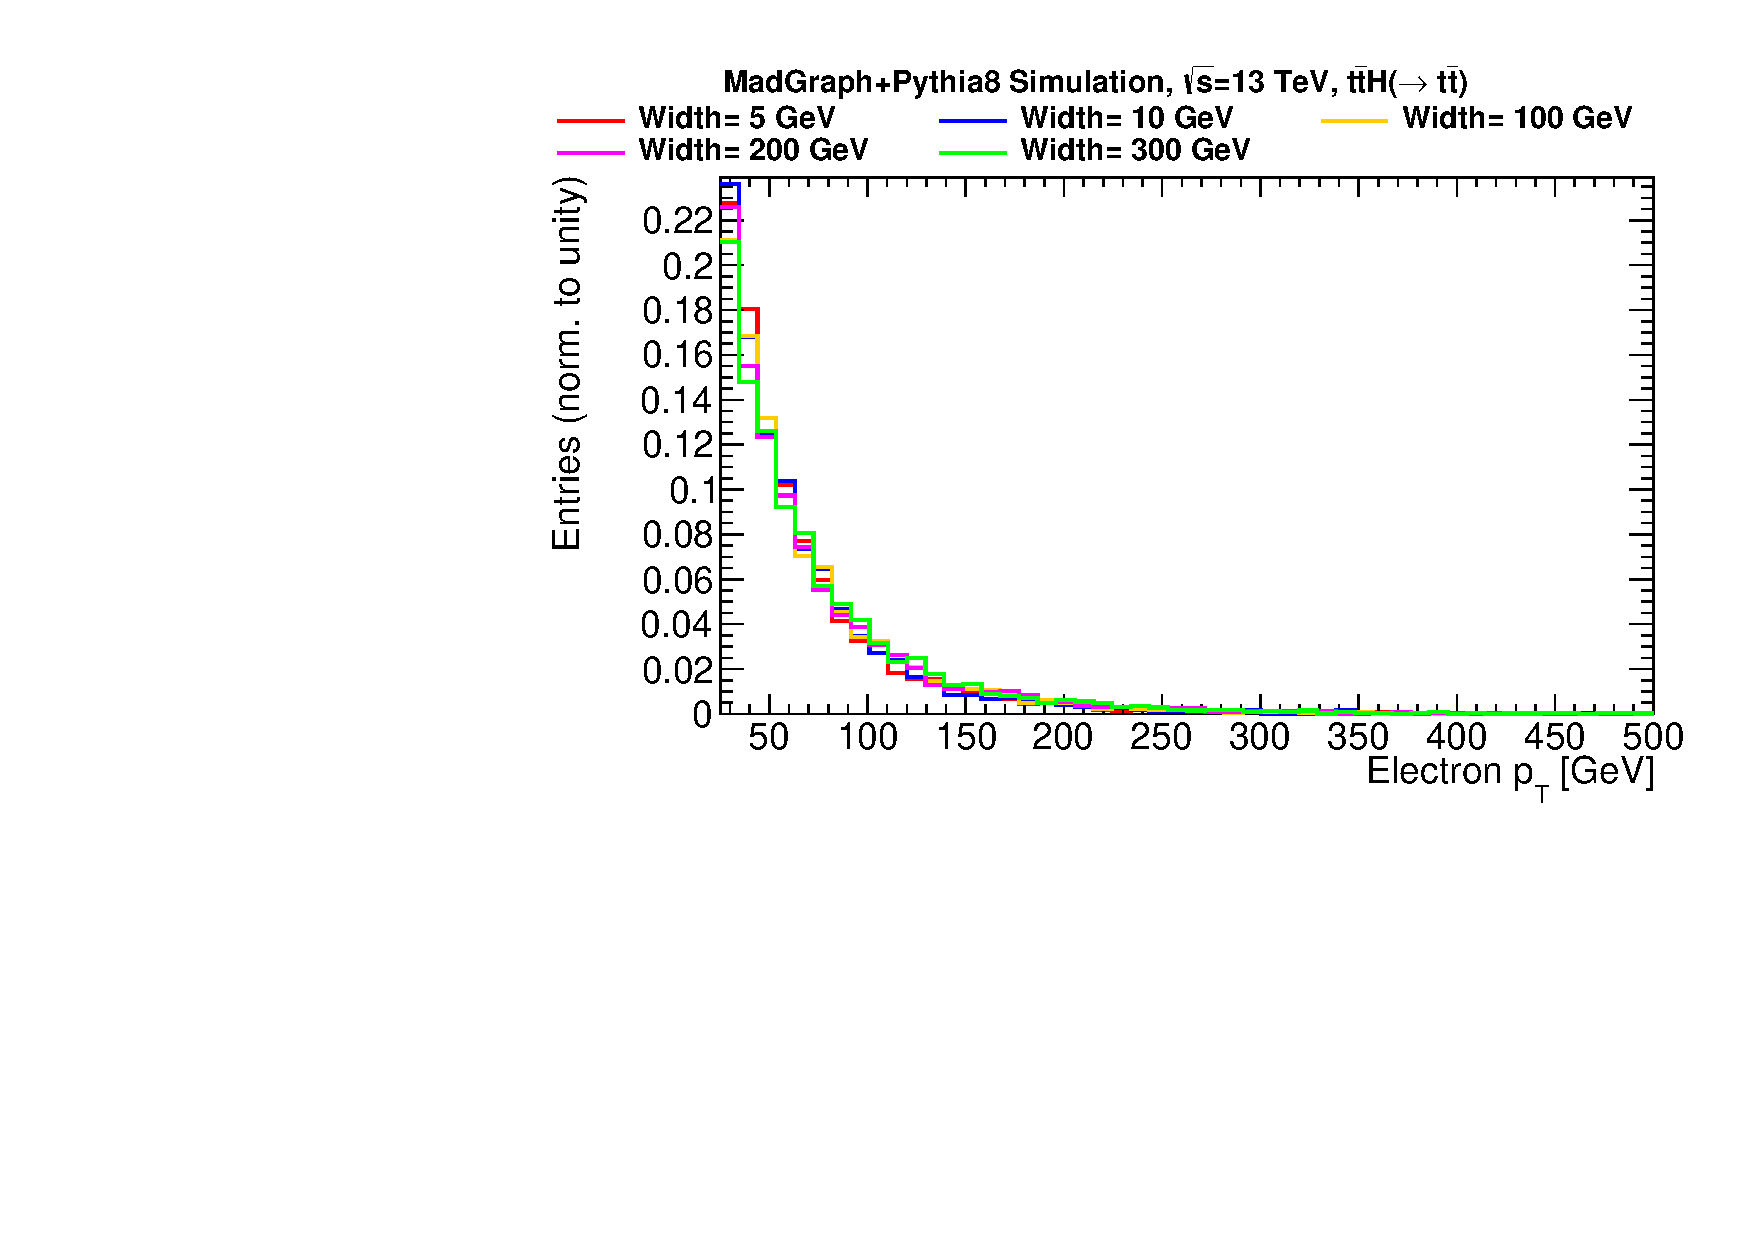
\includegraphics[width=0.43\textwidth]{figures/signal_modeling/width_checks/width_checks_v1_truth_1/plot_n_electrons_pt} &
	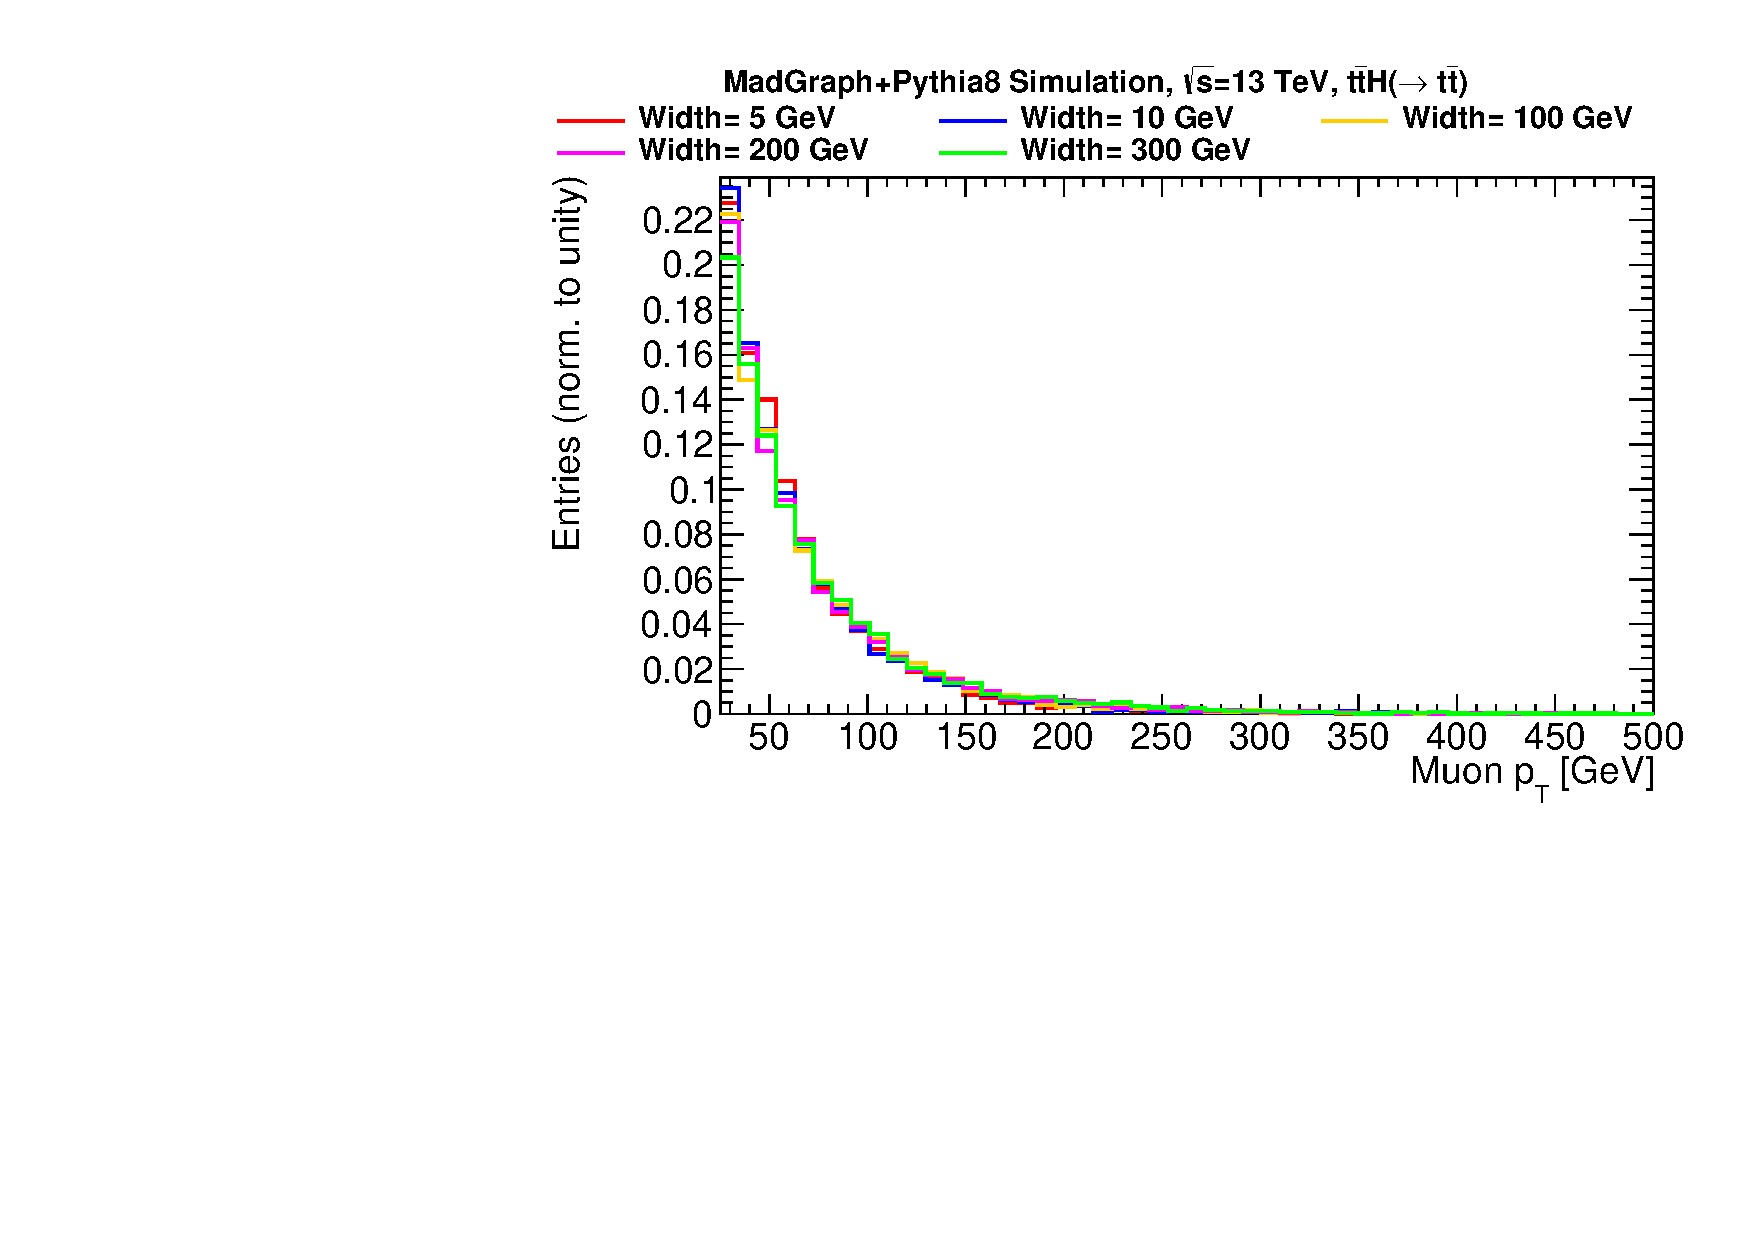
\includegraphics[width=0.43\textwidth]{figures/signal_modeling/width_checks/width_checks_v1_truth_1/plot_n_muons_pt} \\
	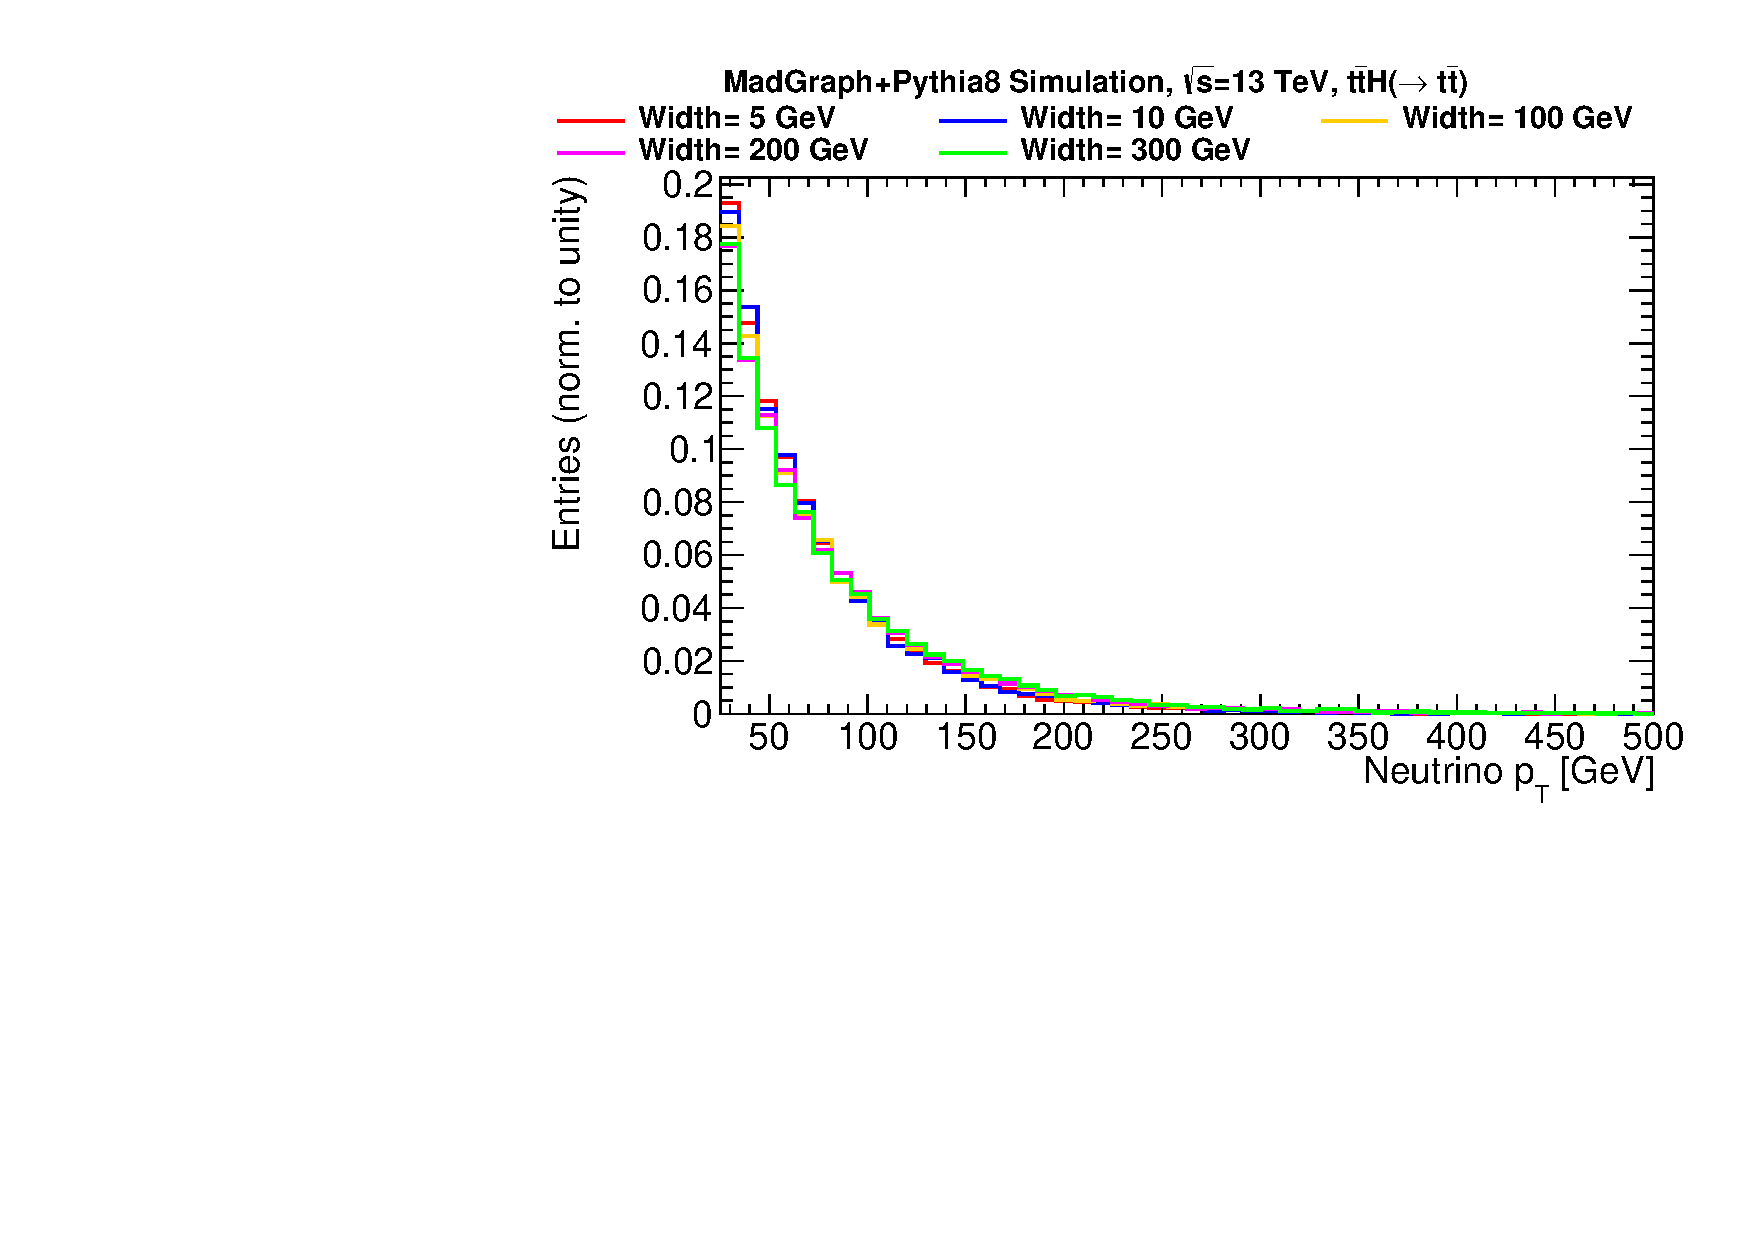
\includegraphics[width=0.43\textwidth]{figures/signal_modeling/width_checks/width_checks_v1_truth_1/plot_n_neutrinos_pt} &
	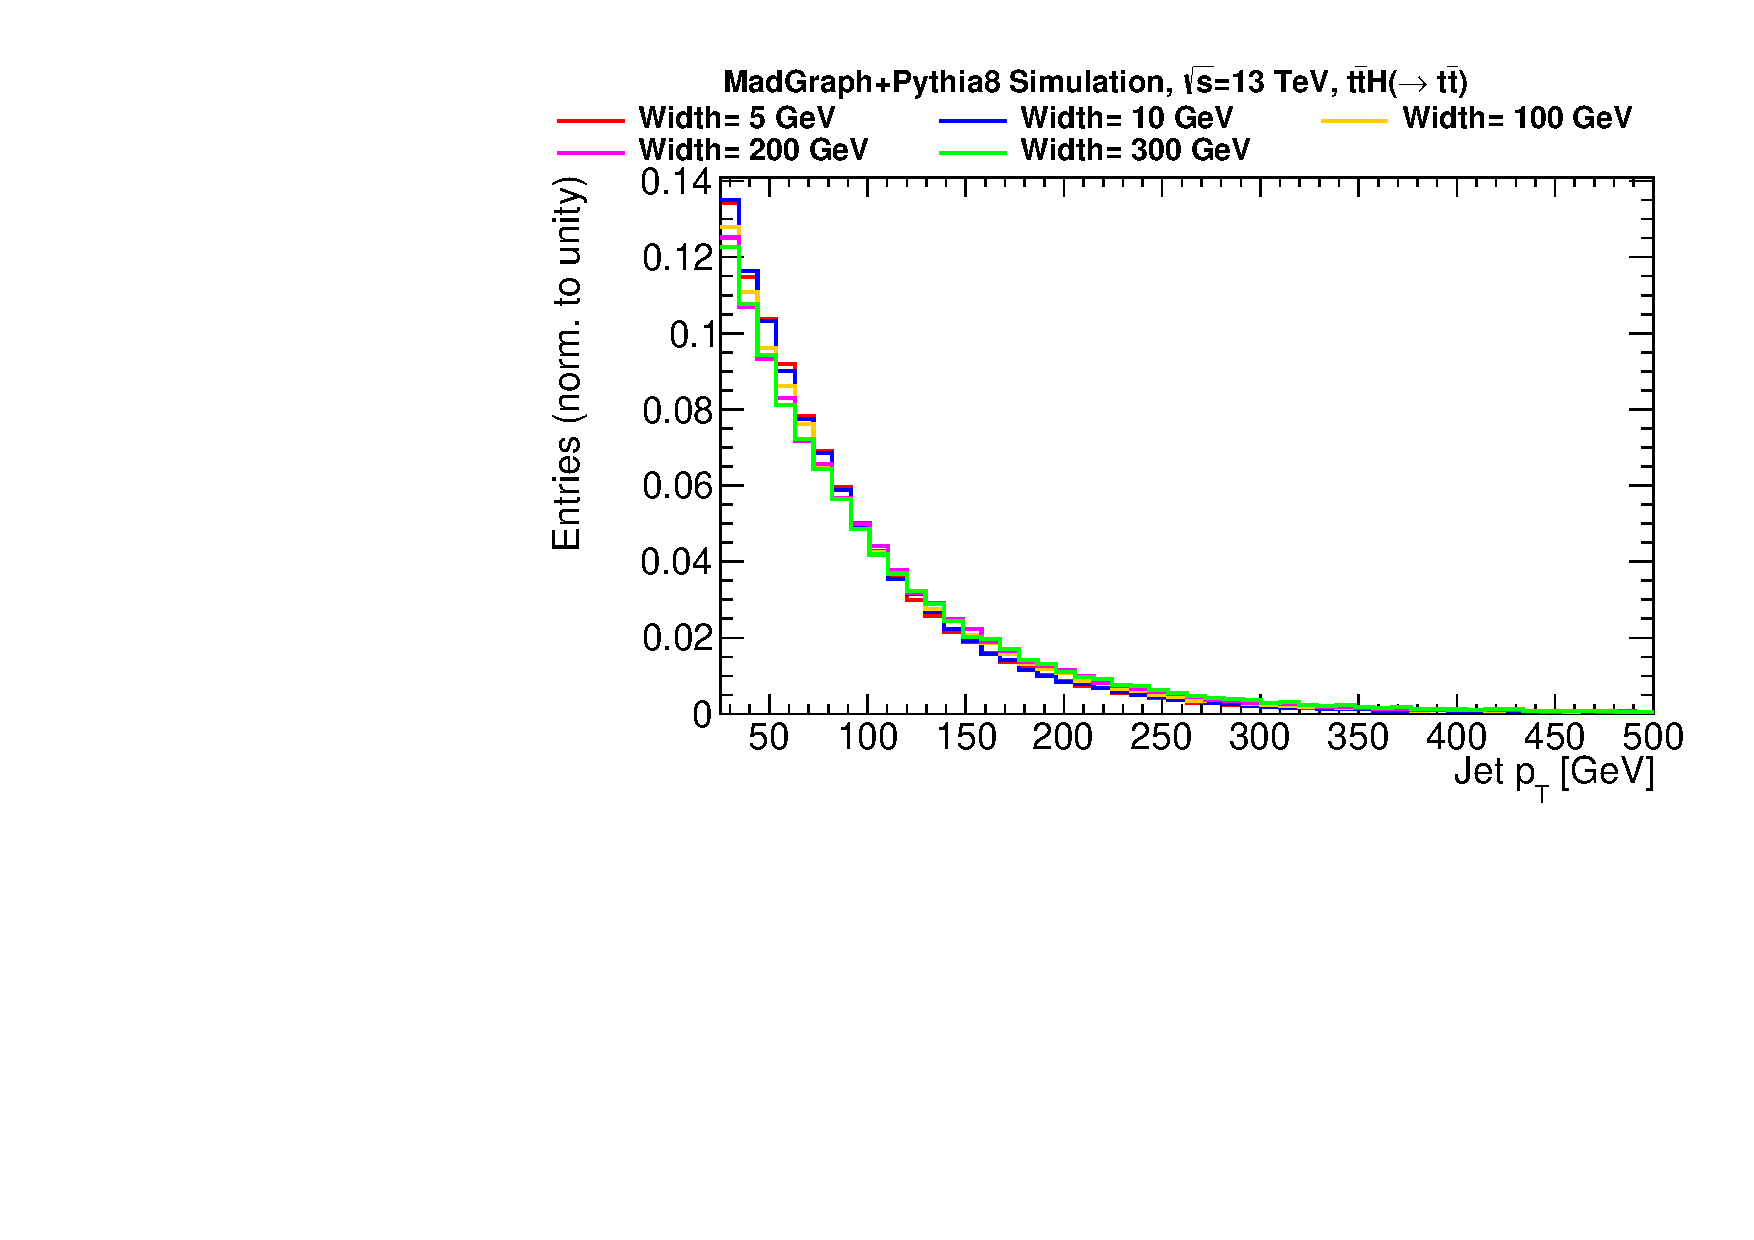
\includegraphics[width=0.43\textwidth]{figures/signal_modeling/width_checks/width_checks_v1_truth_1/plot_n_wzjets_pt} \\
    \end{tabular}
     \caption{Dependence final state particles $p_{T}$ corresponding to different total width values for $m_{H}=400$~GeV. Electrons and Muons are shown at the top, neutrinos and jets at the bottom.}
   \label{figure:2hdm-width-check}
  \end{center}
\end{figure}

The other free parameters of the model don't affect the kinematics and follow the default setting of \MadG.

\begin{table}[!ht]
 \begin{center}\small
    \begin{tabular}{|cccccccccc|}
       \hline
       \multicolumn{10}{|c|}{Mass points [GeV]}\\
        \hline
       200 & 300& 400& 500& 600& 700& 750& 800& 900& 1000\\
       \hline   
       \hline
       \multicolumn{10}{|c|}{Widths [GeV]}\\
        \hline
       1 & 2 & 5& 5& 10& 20& 20& 20& 20& 30\\
       \hline   
\end{tabular}
  \caption{Mass points and widths used for the \ttH\ signal generation.}
  \label{tab:MassWidth}
  \end{center}
\end{table}

\subsection{Interference with the Standard Model background}

Interference effects between the generated BSM signals and the Standard Model background are expected whenever the initial and final state 
particles/partons are the same in the two cases. For the signals introduced in this section, interference might occur with Standard Model four-tops production. 

Studies of the interference effects relevant for this analysis were reported in~\cite{Orlando:2258130}. Interference effects are observed to be at most of the order 
of $20\%$ at parton level, affecting mostly the invariant mass distribution of the Higgs decay products for large width signal scenarios (up to total widths of the order of 100 GeV). Other kinematic distributions, more similar to what used in the final analysis, are affected to a lower extent. As illustration, Figure~\ref{fig:ttHtt:ttfromHm_main} shows  
the invariant mass of the heavy neutral scalar in \ttH\ events with and without taking into account the interference with Standard Model four-top background, 
corresponding to different Higgs boson mass and total width values.  

\begin{figure}[ht]
\begin{center}
\begin{tabular}{ccc}
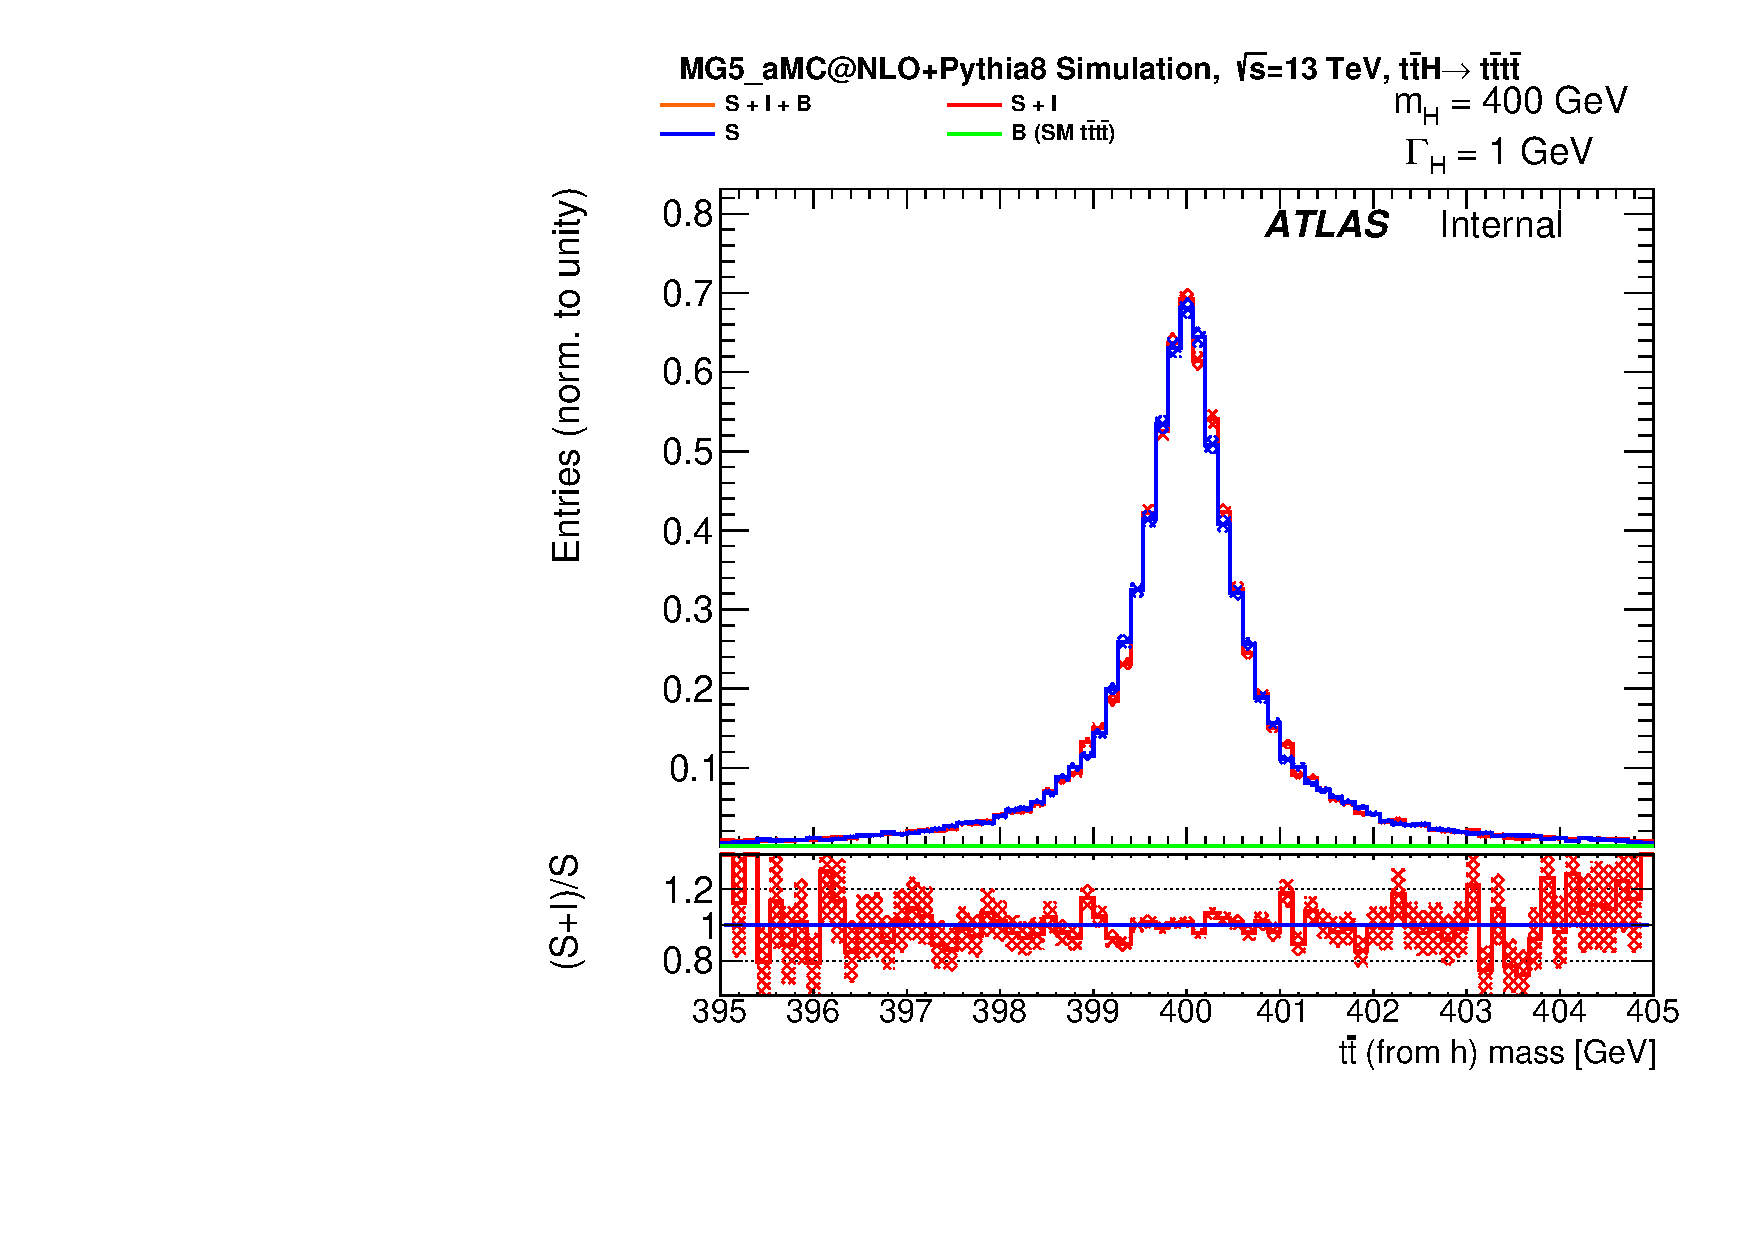
\includegraphics[width=0.315\textwidth]{figures/ttHtt_interf/400_1/plot_n_parton_ttfromH_m.pdf} &

\includegraphics[width=0.315\textwidth]{figures/ttHtt_interf/400_50/plot_n_parton_ttfromH_m.pdf} &

\includegraphics[width=0.315\textwidth]{figures/ttHtt_interf/400_100/plot_n_parton_ttfromH_m.pdf} \\

\includegraphics[width=0.315\textwidth]{figures/ttHtt_interf/500_1/plot_n_parton_ttfromH_m.pdf} &

\includegraphics[width=0.315\textwidth]{figures/ttHtt_interf/500_50/plot_n_parton_ttfromH_m.pdf} &

\includegraphics[width=0.315\textwidth]{figures/ttHtt_interf/500_100/plot_n_parton_ttfromH_m.pdf} \\

\includegraphics[width=0.315\textwidth]{figures/ttHtt_interf/700_1/plot_n_parton_ttfromH_m.pdf} &

\includegraphics[width=0.315\textwidth]{figures/ttHtt_interf/700_50/plot_n_parton_ttfromH_m.pdf} &

\includegraphics[width=0.315\textwidth]{figures/ttHtt_interf/700_100/plot_n_parton_ttfromH_m.pdf} \\

\includegraphics[width=0.315\textwidth]{figures/ttHtt_interf/900_1/plot_n_parton_ttfromH_m.pdf} &

\includegraphics[width=0.315\textwidth]{figures/ttHtt_interf/900_50/plot_n_parton_ttfromH_m.pdf} &

\includegraphics[width=0.315\textwidth]{figures/ttHtt_interf/900_100/plot_n_parton_ttfromH_m.pdf}
\end{tabular}
\caption{Normalized invariant mass distribution of the heavy scalars $H/A$ 
for different width (respectively $1$ GeV (left), $50$ GeV (center) and $100$ GeV (right) ) and mass ($400$ GeV, $500$ GeV, $700$ GeV 
and $900$ GeV, in increasing rows) assumptions. Distributions for signal-only (blue) and signal+interference (red) assumptions are shown (see text). Bands refer to statistical MC uncertainties. The signal is generated assuming $m_{H}=400$~GeV.}
\label{fig:ttHtt:ttfromHm_main}
\end{center}
\end{figure}

Given the limited impact observed on at truth level, no interference effects are considered for this analysis. 

\subsection{Heavy Higgs theoretical predictions}
\label{sec:signal_cross_sections}
The theoretical predictions for the investigated signal processes are described in this sub-section. 
For each mass point available from the generated Monte-Carlo samples, cross sections are evaluated in the relevant parameter-space of the investigated benchmark models.  

The benchmark model we will consider is 2HDM type~II. This model is an ``MSSM-like'' model, in which one Higgs doublet couples to up-type quarks
and the other to down-type quarks and charged leptons. Another common choice from literature is the 2HDM type~I model, but type~I and 
type~II models only differ for their couplings to down-type fermions, thus they predict same cross sections for \ttH\ and \ttA. 

All used cross-sections for heavy neutral Higgs-bosons production are obtained from the standard HBSM recommendations \\
{\small{https://twiki.cern.ch/twiki/bin/viewauth/AtlasProtected/HiggsBSM2HDMRecommendations}} \\
from the LHC HXSG (Higgs Cross-Section working Group). The used version of the cross-sections is 1.6.6\_13TeV; in this version the default cross-sections are derived in the Santander matched 4FS+5FS scheme.

The cross sections in the alignment limit are presented in Fig.~\ref{fig:bench_xsec_ttH_1D}.

\begin{figure}[tbp]
	\begin{center}\setlength{\tabcolsep}{2.0pt}\small   

		\begin{tabular}{cc}
					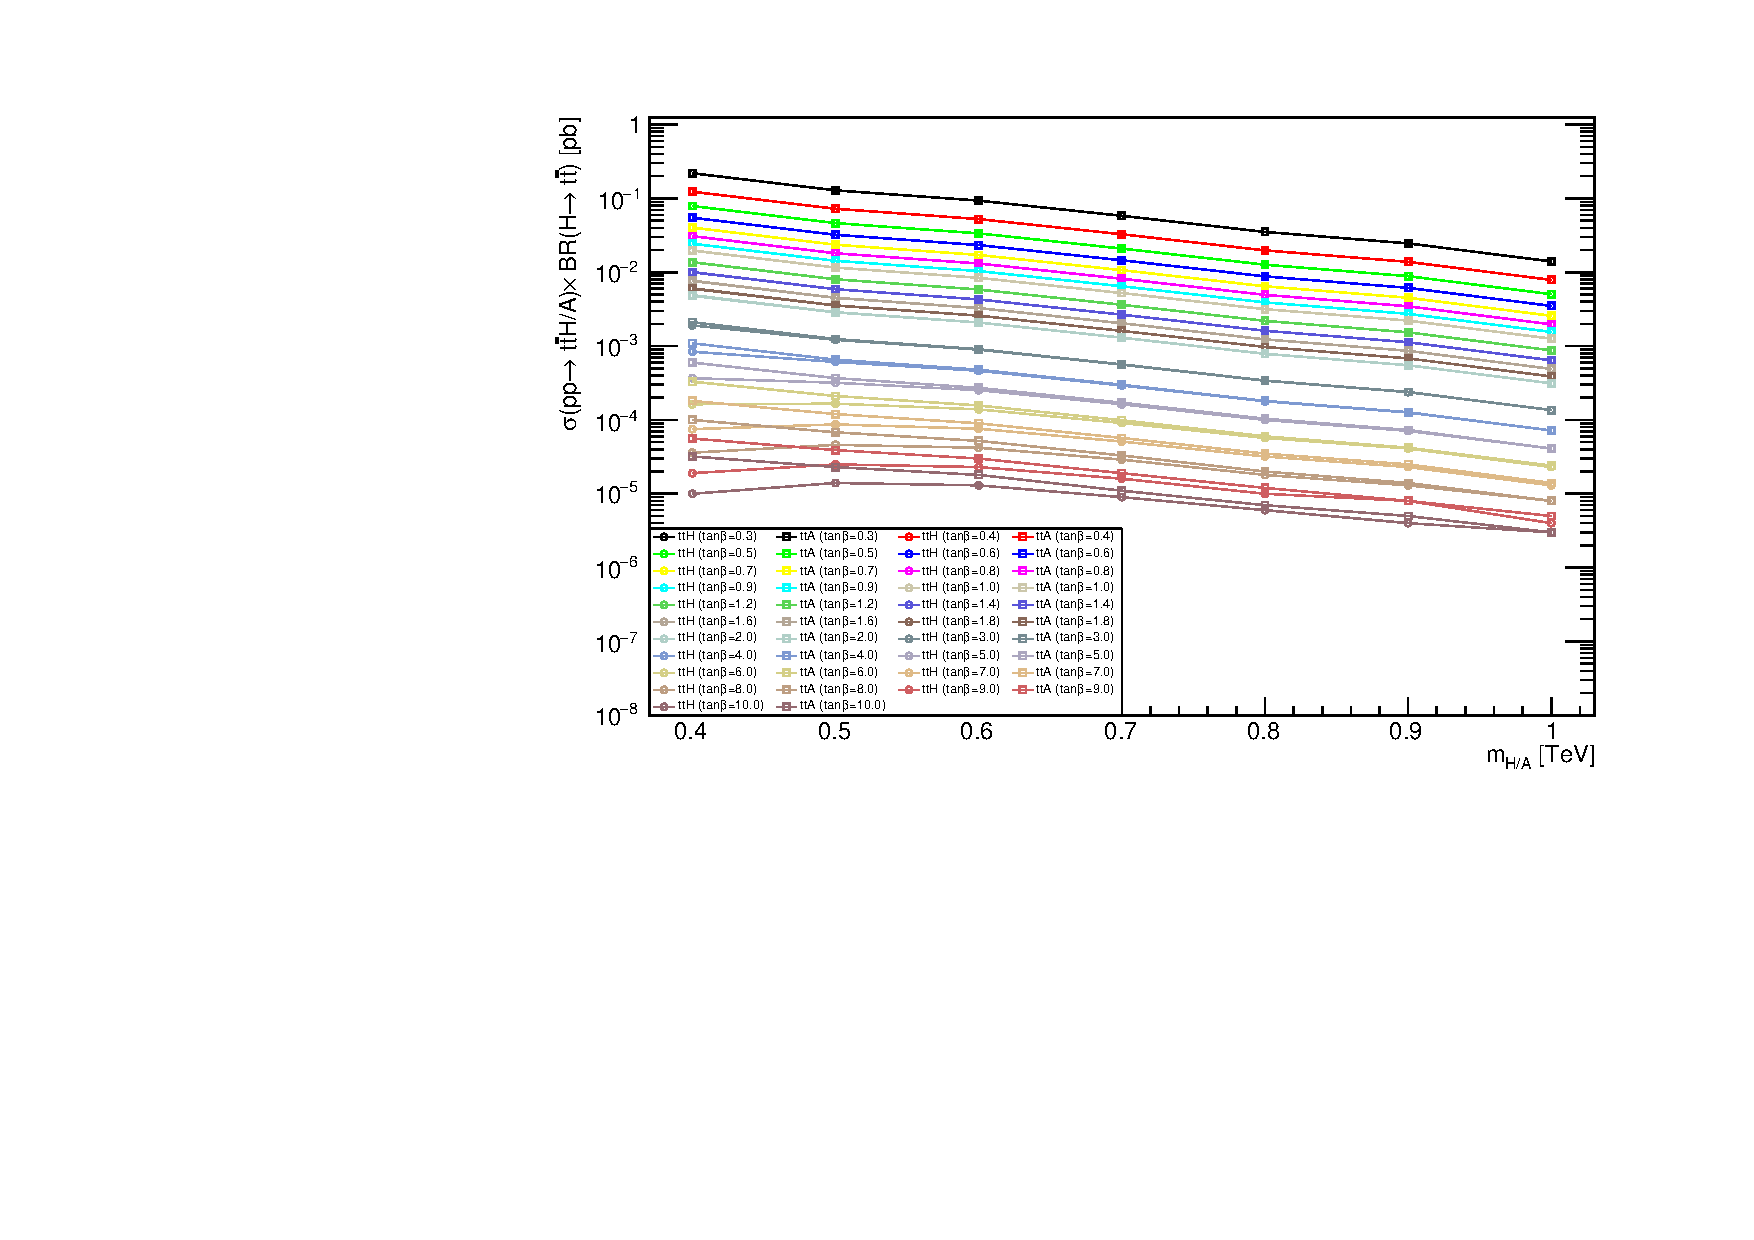
\includegraphics[width=0.47\textwidth]{figures/signal_modeling/hbsm_cross_sections/tanb_mass} 
					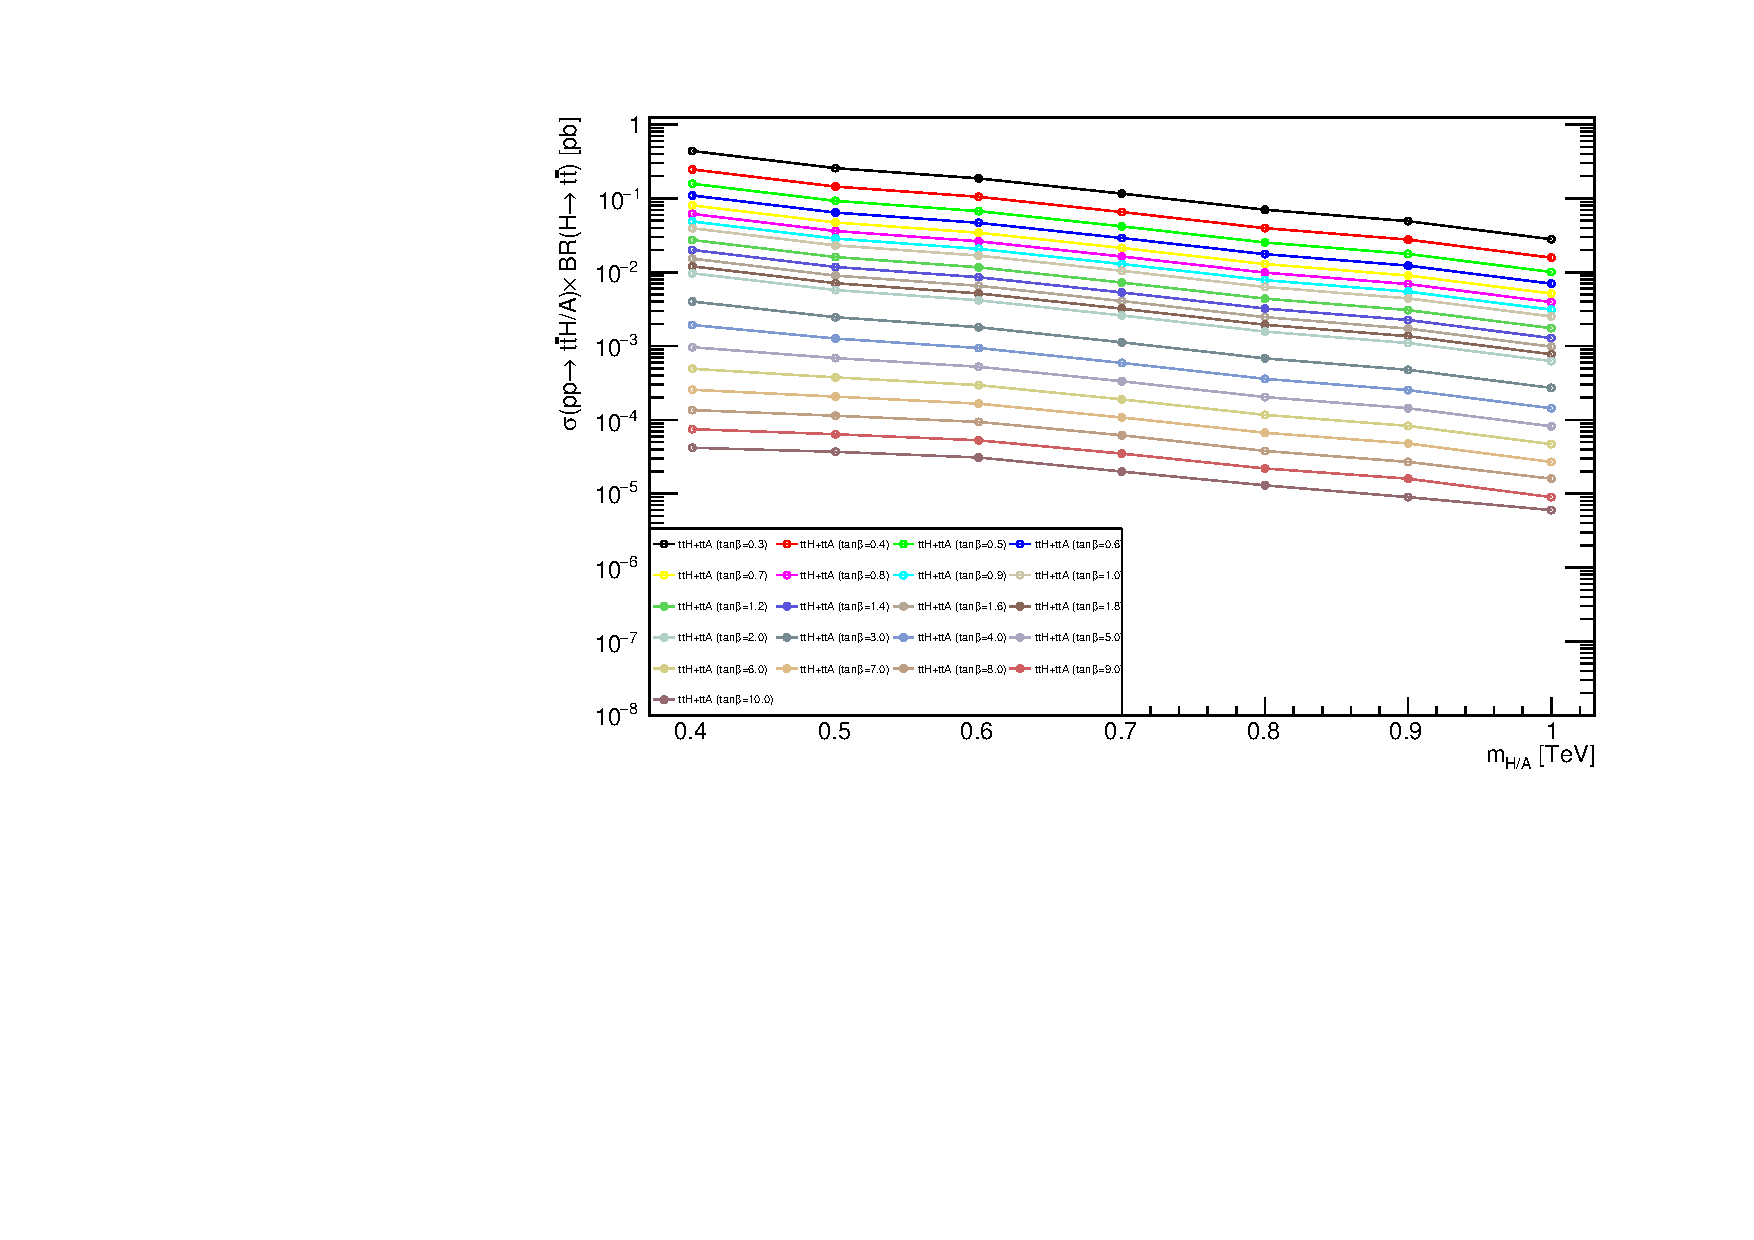
\includegraphics[width=0.47\textwidth]{figures/signal_modeling/hbsm_cross_sections/tanb_mass_merge_ttA_ttH} 
		\end{tabular}
		\caption{Cross-sections times branching-ratios for \ttH\ (left, circle marker), \ttA\ (left, square marker) and $\ensuremath{t\bar{t}H}+\ensuremath{t\bar{t}A}\rightarrow t\bar{t}t\bar{t}$\ (right, circle marker) in 2HDM type~II presented as a funtion of $m_{A}$ for several $\tan\beta$ points in the alignment limit.}
		\label{fig:bench_xsec_ttH_1D}
	\end{center}
\end{figure}



